% ======================================================================
%  AxiSim Software Manual  v1.04-alpha
%  ---------------------------------------------------------------------
%  Drop-in Overleaf project. All diagrams are native TikZ. Screenshots
%  are optional: to enable them in Overleaf, create an "images/" folder
%  and upload the following files. In the repository they already exist
%  under docs/images/ with these names:
%
%     images/sketch.png
%     images/mesh_structured.png
%     images/mesh_unstructured.png
%     images/solver_residuals.png
%     images/results_view.png
%
%  If you do NOT want screenshots yet, set \showscreenshotsfalse below
%  and the figures become captioned placeholders so the document still
%  compiles cleanly.
% ======================================================================
\documentclass[11pt]{article}

\usepackage[margin=1in]{geometry}
\usepackage[T1]{fontenc}
\usepackage{lmodern}
\usepackage{amsmath,amssymb}
\usepackage{graphicx}
\usepackage{booktabs}
\usepackage{array}
\usepackage{xcolor}
\usepackage{subcaption}
\usepackage{enumitem}
\usepackage{listings}
\usepackage{tikz}
\usetikzlibrary{arrows.meta,positioning,calc,shapes.geometric}
\usepackage[hidelinks]{hyperref}

\graphicspath{{images/}}

% ---- toggle screenshots on/off ----
\newif\ifshowscreenshots
\showscreenshotstrue   % <- set to \showscreenshotsfalse to use placeholders

% helper: include a screenshot if enabled, else a placeholder box
\newcommand{\screenshot}[3]{% {file}{width}{placeholder caption}
  \ifshowscreenshots
    \includegraphics[width=#2]{#1}%
  \else
    \fbox{\parbox[c][0.42\textwidth][c]{#2}{\centering\itshape screenshot placeholder:\\ #3}}%
  \fi
}

% ---- listings style for code / console ----
\definecolor{codebg}{RGB}{246,247,249}
\definecolor{codekw}{RGB}{0,90,160}
\definecolor{codecm}{RGB}{110,120,130}
\lstdefinestyle{axisim}{
  backgroundcolor=\color{codebg},
  basicstyle=\ttfamily\small,
  keywordstyle=\color{codekw}\bfseries,
  commentstyle=\color{codecm}\itshape,
  showstringspaces=false,
  breaklines=true,
  frame=single,
  rulecolor=\color{gray!40},
  language=C++,
  morekeywords={struct,uint8_t,double,int,bool,std,vector}
}
\lstset{style=axisim}

\definecolor{warnbg}{RGB}{255,248,225}
\definecolor{warnbd}{RGB}{220,170,40}
\newcommand{\warnbox}[1]{%
  \begin{center}\fcolorbox{warnbd}{warnbg}{\parbox{0.93\linewidth}{#1}}\end{center}}

\title{\textbf{AxiSim Software Manual} \\[2pt] \large GPU-accelerated axisymmetric CFD, from sketch to solution \\[6pt] \normalsize Version 1.04-alpha}
\author{Lui Tsumura}
\date{July 5, 2026}

\begin{document}
\maketitle

\begin{abstract}
\noindent AxiSim is an interactive finite-volume solver for incompressible, axisymmetric
(\(r\text{--}z\)) flow. It combines geometry sketching, structured and unstructured
meshing, a GPU (CUDA) SIMPLE solver, and real-time post-processing in a single
application. This manual documents how to use the software, what it contains, the
algorithms and data structures behind it, and its present limitations. It supersedes
the v1.01 manual and reflects the v1.04-alpha codebase through the July 5, 2026
development snapshot.
\end{abstract}

\tableofcontents
\newpage

% ======================================================================
\section{Introduction}
% ======================================================================
AxiSim is a research/learning CFD application that solves the incompressible
Navier--Stokes equations in axisymmetric coordinates using the finite-volume method
(FVM) and the SIMPLE pressure--velocity coupling scheme. The numerically intensive
work---assembly of discretised equations and the linear solves---runs on an NVIDIA GPU
through CUDA, while the entire workflow (geometry, meshing, solving, and visualisation)
lives in one real-time interface built on OpenGL and Dear ImGui.

The application is organised as a pipeline of stages, each with its own GUI tab, sharing
a common project state:

\begin{figure}[h]
\centering
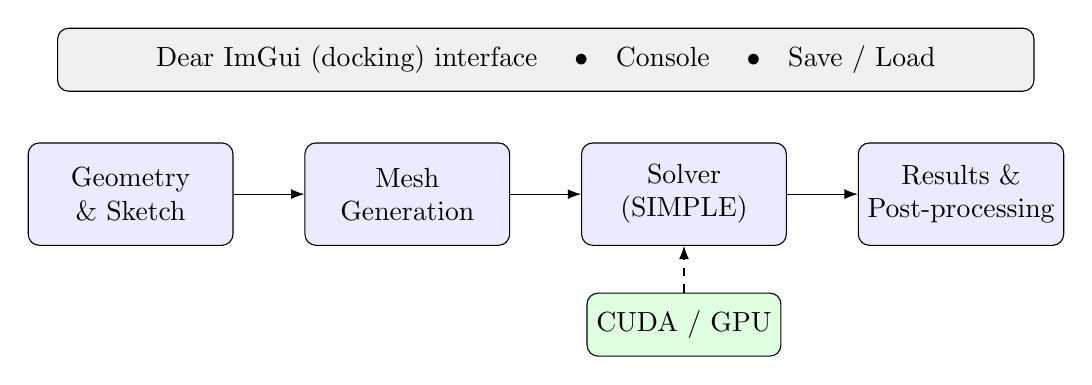
\begin{tikzpicture}[>=Latex,
  stage/.style={draw, rounded corners, minimum width=26mm, minimum height=13mm, align=center, fill=blue!8},
  band/.style={draw, rounded corners, align=center, fill=gray!12, minimum height=8mm}]
  \node[stage](sk){Geometry\\ \& Sketch};
  \node[stage, right=9mm of sk](me){Mesh\\ Generation};
  \node[stage, right=9mm of me](so){Solver\\ (SIMPLE)};
  \node[stage, right=9mm of so](re){Results \&\\ Post-processing};
  \draw[->](sk)--(me); \draw[->](me)--(so); \draw[->](so)--(re);
  \node[band, minimum width=124mm] at ($(sk.north)!0.5!(re.north)+(0,1.05)$)
      {Dear ImGui (docking) interface \quad$\bullet$\quad Console \quad$\bullet$\quad Save / Load};
  \node[band, fill=green!12] at ($(so.south)+(0,-1.0)$) (gpu){CUDA / GPU};
  \draw[->,dashed](gpu)--(so);
\end{tikzpicture}
\caption{High-level architecture. A shared project flows left to right through four
stages; the GUI and console wrap all stages, and the solver offloads to the GPU.}
\label{fig:arch}
\end{figure}

This manual documents the most notable features. Because AxiSim is under active
development, some smaller features may be described only briefly, and details are
subject to change between versions.

% ======================================================================
\section{Disclaimers and Project Status}\label{sec:disclaimer}
% ======================================================================
\warnbox{\textbf{AxiSim is alpha-stage, work-in-progress software. Its numerical results
have not been formally verified or validated. Do not use it for engineering decisions,
safety-critical work, or any application where correctness matters.}}

\subsection{Development status}
AxiSim is at version \texttt{1.04-alpha}. It is updated frequently and changes rapidly;
APIs, file formats, default parameters, and behaviour may change without notice between
versions. Expect rough edges, incomplete features, and the occasional bug.

\subsection{Verification and validation}
The solver has \emph{not} undergone systematic verification (e.g.\ method-of-manufactured-
solutions, grid-convergence studies) or validation against analytical solutions,
trusted reference codes, or experimental data. Results should be treated as
qualitative and exploratory. Known numerical caveats are collected in
Section~\ref{sec:limitations}.

\subsection{Intended use}
AxiSim is intended for learning, prototyping, and experimentation with FVM/CFD and
GPU programming. It is not a substitute for a validated commercial or open-source
solver.

\subsection{Licensing}
The original AxiSim source code is released under the MIT License. However, AxiSim
links the \textbf{Gmsh} library, which is licensed under the GNU GPL v2-or-later.
\emph{Binaries that are built with and distributed alongside Gmsh are therefore
subject to the GPL}, in addition to the MIT terms covering AxiSim's own source. The
third-party components and their licenses are listed in Section~\ref{sec:libraries}.

% ======================================================================
\section{System Requirements and Installation}
% ======================================================================
\subsection{Requirements}
\begin{itemize}[nosep]
  \item \textbf{Operating system:} Windows 10 / 11 (x64).
  \item \textbf{GPU:} an NVIDIA GPU with CUDA compute capability \(\geq 7.5\)
        (Turing / GTX 16 / RTX 20 series and newer) plus a recent driver. AxiSim runs
        its solver on the GPU and \emph{will not run} on machines without a compatible
        NVIDIA card. Release builds must be compiled for the GPU architectures they
        are expected to support.
  \item \textbf{To build from source:} CUDA Toolkit 13.0, a C++20 compiler
        (Visual Studio 2022), CMake \(\geq 3.24\), Ninja, and vcpkg.
\end{itemize}

\subsection{Building from source}
Dependencies that come from vcpkg (GLFW, GLAD, GLM, OpenGL) are installed first; Gmsh
and Dear ImGui/ImPlot are bundled in the repository. The repository currently includes
\texttt{CMakeSettings.json} for Visual Studio's CMake integration. If configuring from
the command line, use the vcpkg toolchain file explicitly:
\begin{lstlisting}[language={}]
vcpkg install glfw3 glad glm
cmake -S . -B out/build/x64-Release -G Ninja ^
  -DCMAKE_BUILD_TYPE=RelWithDebInfo ^
  -DCMAKE_TOOLCHAIN_FILE=<path-to-vcpkg>/scripts/buildsystems/vcpkg.cmake
cmake --build out/build/x64-Release --target AxiSim
\end{lstlisting}

\warnbox{\textbf{CUDA architecture note.} The checked-in CMake file currently targets
\texttt{CUDA\_ARCHITECTURES "86-real"} for a local Ampere development GPU. For a
redistributable build, change this list to include the architectures you intend to
support (for example Turing/Ampere/Ada plus a PTX fallback). Otherwise the produced
binary may only run on matching GPUs even though the source code targets CUDA-capable
hardware more broadly.}

\subsection{Runtime files}
The executable loads several resources by relative path, so the following must sit
next to \texttt{AxiSim.exe} when distributing or running outside the build tree:
\texttt{glfw3.dll}, \texttt{gmsh-4.15.dll}, the \texttt{assets/} folder (fonts and
icons), and the \texttt{graphics/shaders/} folder. The CUDA runtime is statically
linked, so end users do not need the CUDA Toolkit---only an NVIDIA driver. The Visual
C++ runtime (\texttt{MSVCP140.dll}, \texttt{VCRUNTIME140*.dll}) must be present (install
the Microsoft Visual C++ Redistributable x64 if needed).

\subsection{Packaging a release ZIP}
The \texttt{package.ps1} script builds the \texttt{AxiSim} target, installs it into a
staging directory, checks for required runtime assets, and writes a ZIP under
\texttt{dist/}. A typical release-package command is:
\begin{lstlisting}[language={}]
.\package.ps1 -Version v1.04-alpha
\end{lstlisting}
Use \texttt{-SkipBuild} only when the chosen build directory already contains a fresh
successful build. The package still cannot include the user's NVIDIA driver; target
machines need a compatible driver and GPU.

% ======================================================================
\section{Libraries and Dependencies}\label{sec:libraries}
% ======================================================================
Table~\ref{tab:libs} lists the notable external components used by AxiSim.

\begin{table}[h]
\centering
\caption{External libraries and their roles.}
\label{tab:libs}
\begin{tabular}{@{}>{\raggedright\arraybackslash}p{0.20\linewidth}
                   >{\raggedright\arraybackslash}p{0.52\linewidth}
                   >{\raggedright\arraybackslash}p{0.20\linewidth}@{}}
\toprule
\textbf{Library} & \textbf{Role in AxiSim} & \textbf{License} \\
\midrule
OpenGL              & Graphics API for creating the window and rendering models       & system \\
GLSL                & Shading language used with OpenGL to render onto the screen      & (OpenGL) \\
GLFW                & Window creation, OS context, and input handling                  & zlib/libpng \\
GLAD                & OpenGL function loader                                            & MIT/public \\
GLM                 & Vector / matrix / quaternion math (camera, transforms)           & MIT \\
Dear ImGui (docking)& Main GUI library; docking branch for dockable windows           & MIT \\
ImPlot              & Real-time plotting (residual plots)                              & MIT \\
Gmsh                & Unstructured (triangular) mesh generation                        & \textbf{GPL v2+} \\
stb\_image          & Loading PNG icon/texture assets                                  & MIT/public \\
NVIDIA CUDA Toolkit & GPU compute: assembly and linear solvers                         & NVIDIA EULA \\
\bottomrule
\end{tabular}
\end{table}

\noindent See Section~\ref{sec:disclaimer} for the licensing consequence of linking Gmsh.

% ======================================================================
\section{What Is Included: Application Overview}
% ======================================================================
AxiSim ships as a single application whose major components are:
\begin{itemize}[nosep]
  \item \textbf{Geometry / Sketch view} --- draw the axisymmetric cross-section
        (lines, rectangles, circles, arcs) with live dimensions, snapping, trim,
        erase, select/move, and undo/redo.
  \item \textbf{Mesh Inspector} --- convert the sketch into a structured (Cartesian)
        or unstructured (Gmsh) mesh, define boundary groups, add local refinement
        regions, and inspect per-cell mesh data.
  \item \textbf{Solver} --- configure and run the SIMPLE solver; choose discretisation
        schemes, relaxation, steady/transient mode, and optional scalar transport.
  \item \textbf{Results} --- 3D revolved field visualisation and a 2D cross-section
        inspector with colormaps and a colorbar.
  \item \textbf{Console} --- text commands to drive major operations and settings.
  \item \textbf{Residual plot} --- live convergence monitoring via ImPlot.
  \item \textbf{Save / Load} --- persist and reload project state through the File
        menu or console commands.
\end{itemize}

A typical end-to-end session follows the workflow in Figure~\ref{fig:workflow}.

\begin{figure}[h]
\centering
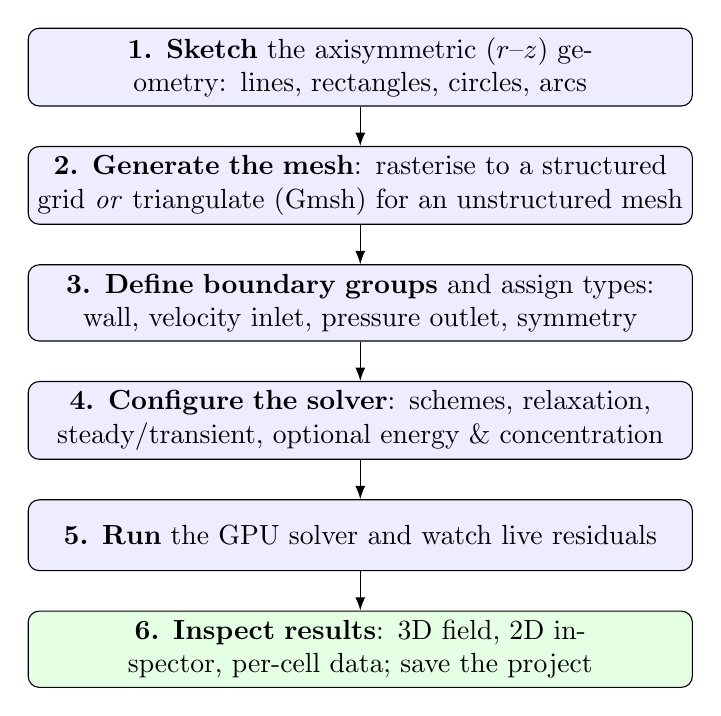
\begin{tikzpicture}[>=Latex, node distance=5mm,
  wfbox/.style={draw, rounded corners, align=center, text width=82mm, minimum height=9mm, fill=blue!7}]
  \node[wfbox](s1){\textbf{1. Sketch} the axisymmetric ($r$--$z$) geometry: lines, rectangles, circles, arcs};
  \node[wfbox, below=of s1](s2){\textbf{2. Generate the mesh}: rasterise to a structured grid \emph{or} triangulate (Gmsh) for an unstructured mesh};
  \node[wfbox, below=of s2](s3){\textbf{3. Define boundary groups} and assign types: wall, velocity inlet, pressure outlet, symmetry};
  \node[wfbox, below=of s3](s4){\textbf{4. Configure the solver}: schemes, relaxation, steady/transient, optional energy \& concentration};
  \node[wfbox, below=of s4](s5){\textbf{5. Run} the GPU solver and watch live residuals};
  \node[wfbox, below=of s5, fill=green!10](s6){\textbf{6. Inspect results}: 3D field, 2D inspector, per-cell data; save the project};
  \foreach \a/\b in {s1/s2,s2/s3,s3/s4,s4/s5,s5/s6}{\draw[->](\a)--(\b);}
\end{tikzpicture}
\caption{The typical AxiSim workflow.}
\label{fig:workflow}
\end{figure}

% ======================================================================
\section{Getting Started: A Typical Workflow}
% ======================================================================
\subsection{Sketching the geometry}
The geometry view lets you draw the cross-section of the axisymmetric domain in the
\((z, r)\) half-plane. Supported primitives are lines, rectangles, circles, and arcs,
with live dimensioning and snapping to existing geometry, the axes, grid vertices, and
the origin. The toolbar includes reset-view, dimension, trim, erase, line, rectangle,
circle, grid display, and copy-to-clipboard controls. Selection supports single clicks,
box selection, moving selected segments, undo/redo, and editable dimension labels. A
2D camera (pan with the middle mouse button, zoom with the wheel) frames the sketch.

\begin{figure}[h]
\centering
\screenshot{sketch.png}{0.8\linewidth}{geometry sketching view}
\caption{Sketching the axisymmetric cross-section.}
\label{fig:sketch}
\end{figure}

\subsection{Generating the mesh}
With a closed sketch, the Mesh Inspector converts the geometry into a finite-volume
mesh (Section~\ref{sec:mesh}). Choose either a structured Cartesian mesh or an
unstructured triangular mesh in the Mesh tab, then press \textbf{Generate Mesh}.
Boundary segments are detected automatically and can be grouped and named for
boundary-condition assignment. If no sketch geometry exists, the mesh generator falls
back to a simple default domain so the rest of the workflow can still be exercised.

\subsection{Defining boundaries and running}
Assign a boundary type to each named group, configure the solver
(Section~\ref{sec:solver}), and run. The residual plot updates live so you can monitor
convergence. When the run finishes, switch to the Results tab to explore the field.

\subsection{Saving the project}
Use \textbf{File \(\rightarrow\) Save}, \textbf{File \(\rightarrow\) Save As}, or
\texttt{save project} in the console to persist the whole project. Use
\textbf{File \(\rightarrow\) Open Project} or \texttt{load project} to reload it. The
File menu can also mark the current project as the one to reopen at startup.

% ======================================================================
\section{Mesh Generation}\label{sec:mesh}
% ======================================================================
AxiSim supports two mesh families, both reduced to a common finite-volume
representation (Section~\ref{sec:fvdata}).

\subsection{Structured mesh}
The structured mesh is a Cartesian grid in the \((z, r)\) plane defined by the number of
cells \(n_z\) and \(n_r\), the domain length \(L\) and radius \(R\), and optional axial/
radial grading (\texttt{zBias}, \texttt{rBias}). The sketch is \emph{rasterised} onto this
grid: every cell whose centre lies outside the sketched domain (or inside an obstacle)
is flagged solid. This is recorded in \texttt{activeCell} (1 = fluid, 0 = solid) and the
set \texttt{obstacleIndices}. Cell index ordering is row-major, \(n = i\,n_z + j\), where
\(i\) is the radial index and \(j\) the axial index. In v1.04-alpha, sketch-to-structured
conversion first reconstructs the closed sketch loops, then uses those loops to set the
structured domain extents and active cells.

\subsection{Unstructured mesh}
The unstructured mesh is a constrained Delaunay triangulation produced by Gmsh from the
sketch boundary. Local refinement is controlled by \emph{regions of influence}
(rectangular or circular), which set a target element size inside the region and a
transition to the background size outside it. Boundary sizing (edge count / target
spacing / bias) can be set per boundary segment or group. Each triangle becomes one
finite-volume cell. Sketch rectangles, circles, and arcs are sampled into boundary
segments before triangulation; the outermost closed loop is treated as the domain and
inner loops become obstacles.

\begin{figure}[h]
\centering
\begin{subfigure}{0.48\linewidth}\centering
  \screenshot{mesh_structured.png}{\linewidth}{structured mesh}
  \caption{Structured (Cartesian) mesh.}
\end{subfigure}\hfill
\begin{subfigure}{0.48\linewidth}\centering
  \screenshot{mesh_unstructured.png}{\linewidth}{unstructured mesh}
  \caption{Unstructured (Gmsh) mesh.}
\end{subfigure}
\caption{The two meshing modes.}
\label{fig:meshes}
\end{figure}

\subsection{Finite-volume data structure}\label{sec:fvdata}
Regardless of mesh family, the solver consumes a single \texttt{FVMesh} made of cells and
faces. A cell stores its centroid, 2D area, revolved volume \(V = 2\pi r_c A_{2D}\)
(axisymmetric), and the IDs of its bounding faces. A face stores its owner and neighbour
cell, its outward unit normal, its centre, and its (revolved) area; a face with
\texttt{neighbor} \(= -1\) is a boundary face.

\begin{lstlisting}
struct FVCell {
    Vec2 center;          // centroid (z, r)
    double area2D = 0.0;  // 2D cross-sectional area
    double volume = 0.0;  // revolved volume 2*pi*r_c*area2D
    std::vector<int> faceIDs;
    bool active = true;   // false => solid / excluded
    bool solid  = false;
};

struct FVFace {
    int owner = -1, neighbor = -1;  // neighbor < 0  => boundary face
    int v0 = -1, v1 = -1;           // edge endpoints
    Vec2 normal, center;            // outward unit normal; face midpoint
    double length2D = 0.0, area = 0.0;
    int boundaryGroupID = -1;
};
\end{lstlisting}

Figure~\ref{fig:fvcell} shows two adjacent (triangular) cells, the owner $P$ and
neighbour $N$, the centroid-to-centroid vector $\mathbf{d}$, and the face outward
normal $\mathbf{S}$. These two quantities drive both the diffusion discretisation and
the mesh-quality measure below.

\begin{figure}[h]
\centering
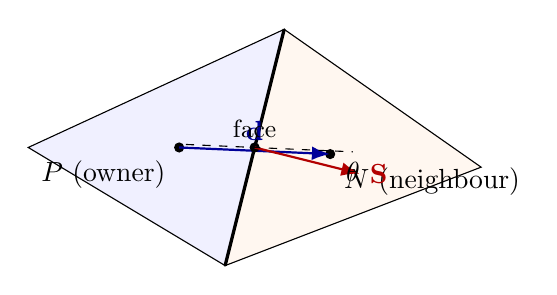
\begin{tikzpicture}[>=Latex, scale=1.25,
  dot/.style={circle, fill=black, inner sep=1.3pt}]
  \coordinate (F1) at (2,0);
  \coordinate (F2) at (2.6,2.4);
  \coordinate (PL) at (0,1.2);
  \coordinate (NR) at (4.6,1.0);
  \draw[fill=blue!6]   (F1)--(F2)--(PL)--cycle;
  \draw[fill=orange!6] (F1)--(F2)--(NR)--cycle;
  \draw[very thick] (F1)--(F2);
  \coordinate (P) at (1.533,1.2);
  \coordinate (N) at (3.067,1.133);
  \node[dot,label=below left:{$P$ (owner)}] at (P){};
  \node[dot,label=below right:{$N$ (neighbour)}] at (N){};
  \draw[->,thick,blue!60!black] (P)--(N) node[midway,above]{$\mathbf{d}$};
  \coordinate (Fm) at (2.3,1.2);
  \node[dot] at (Fm){};
  \draw[->,thick,red!70!black] (Fm)--($(Fm)+(1.066,-0.266)$) node[right]{$\mathbf{S}$};
  \draw[dashed] (1.601,1.231)--(3.299,1.156);
  \node at (3.30,0.95){$\theta$};
  \node[above] at (Fm){\small face};
\end{tikzpicture}
\caption{Two adjacent finite-volume cells. $\mathbf{d}$ joins the cell centroids and
$\mathbf{S}$ is the shared-face outward normal. The angle $\theta$ between them is the
\emph{non-orthogonality} (zero for a perfectly orthogonal mesh).}
\label{fig:fvcell}
\end{figure}

\subsection{Boundary groups}
Boundary faces are organised into named \emph{boundary groups}. Domain edges and
obstacle edges are detected, merged into segments, and the user groups and names them.
Each group carries a boundary type and per-field values that the solver reads when
applying boundary conditions (Section~\ref{sec:bc}). Groups also store orientation
metadata, total boundary length, optional boundary sizing, and optional scalar wall
layers. For structured meshes, groups retain a lookup to their grid edges; for
unstructured meshes, groups are resolved through boundary vertices, edges, and
segments.

\subsection{Regions of influence}
Regions of influence are local mesh-sizing controls for unstructured meshes. A region
may be circular or rectangular, enabled/disabled independently, and configured with a
target spacing, outside spacing, and transition thickness. They are useful for
concentrating triangles around inlets, outlets, wall-reaction zones, or other areas
where stronger gradients are expected. Regions are saved with the project.

\subsection{Mesh quality: non-orthogonality}\label{sec:nonortho}
For each interior face, the non-orthogonality angle is
\begin{equation}
\theta = \arccos\!\left(\frac{\mathbf{d}\cdot\mathbf{S}}{\lvert\mathbf{d}\rvert\,\lvert\mathbf{S}\rvert}\right),
\end{equation}
where $\mathbf{d}$ is the owner-to-neighbour centroid vector and $\mathbf{S}$ the face
normal. A value of $0^\circ$ means the centroid line is parallel to the face normal
(ideal); larger angles increase discretisation error and can slow or destabilise the
solve. The Mesh Inspector's cell-pick tool reports each cell's centroid, area/volume,
face count, per-face neighbour and length, and the per-cell maximum and average
non-orthogonality. Structured cells report $\approx 0^\circ$ (a useful sanity check),
while skewed triangles report larger values.

% ======================================================================
\section{Solver}\label{sec:solver}
% ======================================================================
\subsection{Governing equations}
AxiSim solves the steady or unsteady incompressible Navier--Stokes equations in
axisymmetric \((z, r)\) coordinates (no swirl). Continuity and momentum are
\begin{align}
\frac{\partial u_z}{\partial z} + \frac{1}{r}\frac{\partial (r\,u_r)}{\partial r} &= 0, \\[4pt]
\rho\,\frac{D u_z}{Dt} &= -\frac{\partial p}{\partial z}
   + \mu\!\left[\frac{\partial^2 u_z}{\partial z^2} + \frac{1}{r}\frac{\partial}{\partial r}\!\left(r\,\frac{\partial u_z}{\partial r}\right)\right], \\[4pt]
\rho\,\frac{D u_r}{Dt} &= -\frac{\partial p}{\partial r}
   + \mu\!\left[\frac{\partial^2 u_r}{\partial z^2} + \frac{\partial}{\partial r}\!\left(\frac{1}{r}\frac{\partial (r\,u_r)}{\partial r}\right)\right].
\end{align}
Optional passive scalars---temperature \(T\) (energy) and concentration \(C\)---are
transported by convection--diffusion equations and can be enabled independently
(\texttt{solveEnergy}, \texttt{solveConcentration}). The scalars are solved after the
momentum/pressure update within the SIMPLE iteration. The concentration solver also
supports reactive wall-consumption boundary conditions.

\subsection{Scalar transport and wall reactions}
The scalar equations use the same finite-volume mesh and optional convection term as
the momentum equations. In compact form:
\begin{align}
\frac{\partial T}{\partial t} + \nabla\cdot(\mathbf{u}T)
  &= \nabla\cdot(\alpha_T\nabla T), \qquad
     \alpha_T = \frac{k}{\rho c_p}, \\
\frac{\partial C}{\partial t} + \nabla\cdot(\mathbf{u}C)
  &= \nabla\cdot(D\nabla C).
\end{align}
For concentration walls, v1.04-alpha includes Michaelis--Menten and Hill kinetic
conditions. The wall concentration \(C_w\) is found from a transfer balance between the
cell value \(C_P\), the cell-to-face diffusion resistance, any user-entered wall-layer
resistance, and the reaction flux:
\begin{equation}
h(C_P - C_w) = J(C_w).
\end{equation}
For Michaelis--Menten kinetics,
\begin{equation}
J_{MM}(C_w)=\frac{V_{\max} C_w}{K_m + C_w}\,I(C_w),
\end{equation}
and for Hill kinetics,
\begin{equation}
J_H(C_w)=\frac{V_{\max} C_w^n}{K_m^n + C_w^n}\,I(C_w).
\end{equation}
The optional inhibition factor is
\begin{equation}
I(C_w)=1-\frac{V_2 C_w^m}{K_2^m + C_w^m},
\end{equation}
and is disabled by setting \(V_2=0\). The solver uses Newton iterations on the GPU to
solve the wall balance and clamps negative wall concentrations to zero.

\subsection{The SIMPLE algorithm}
Pressure--velocity coupling uses SIMPLE (Semi-Implicit Method for Pressure-Linked
Equations). Each outer iteration solves under-relaxed momentum predictors, then a
pressure-correction equation, then corrects velocity, pressure, and the face mass flux
(Figure~\ref{fig:simple}). Under-relaxation is required for stability; the defaults are
momentum \(\approx 0.7\) and pressure \(\approx 0.3\).

\begin{figure}[h]
\centering
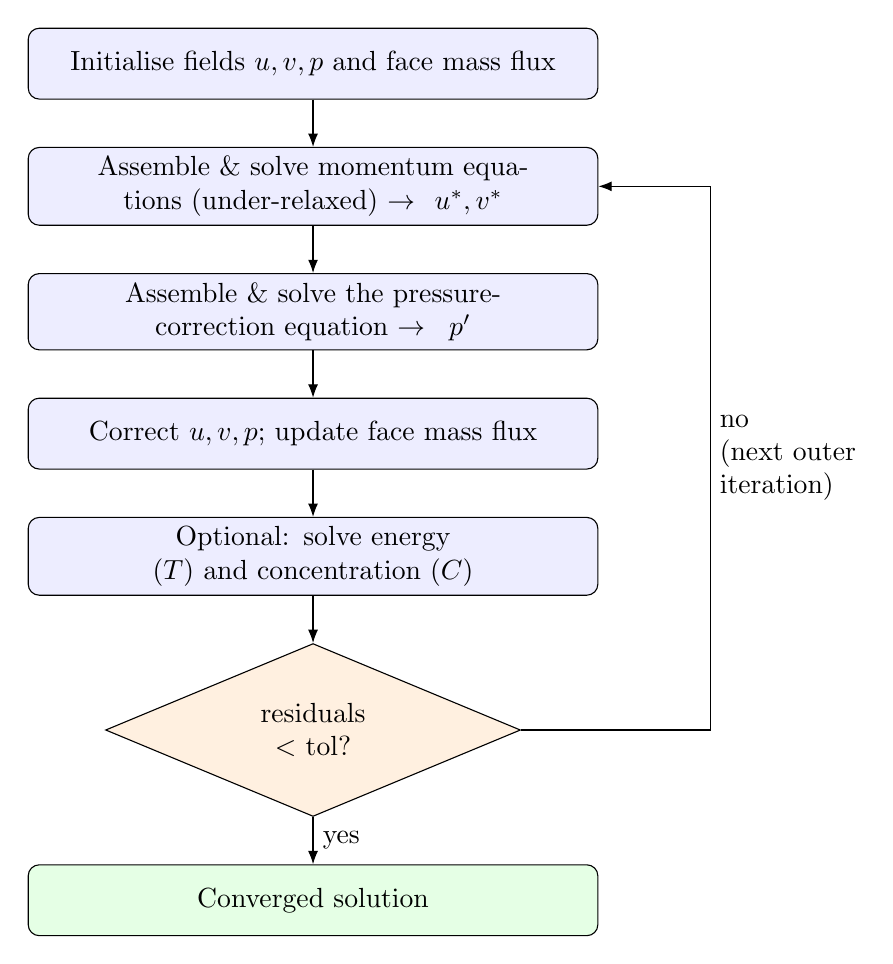
\begin{tikzpicture}[>=Latex, node distance=6mm,
  box/.style={draw, rounded corners, align=center, text width=70mm, minimum height=9mm, fill=blue!7},
  dec/.style={draw, diamond, aspect=2.4, align=center, fill=orange!12, inner sep=1pt, text width=34mm}]
  \node[box](init){Initialise fields $u,v,p$ and face mass flux};
  \node[box,below=of init](mom){Assemble \& solve momentum equations (under-relaxed) $\rightarrow u^{*}, v^{*}$};
  \node[box,below=of mom](pp){Assemble \& solve the pressure-correction equation $\rightarrow p'$};
  \node[box,below=of pp](corr){Correct $u, v, p$; update face mass flux};
  \node[box,below=of corr](scal){Optional: solve energy ($T$) and concentration ($C$)};
  \node[dec,below=of scal](conv){residuals\\ $<$ tol?};
  \node[box,below=of conv, fill=green!10](done){Converged solution};
  \draw[->](init)--(mom); \draw[->](mom)--(pp); \draw[->](pp)--(corr);
  \draw[->](corr)--(scal); \draw[->](scal)--(conv);
  \draw[->](conv)--node[right]{yes}(done);
  \draw[->](conv.east) -- ++(2.4,0) |- node[pos=0.25,right,align=left]{no\\ (next outer\\ iteration)} (mom.east);
\end{tikzpicture}
\caption{One outer iteration of the SIMPLE loop as implemented in AxiSim.}
\label{fig:simple}
\end{figure}

\subsection{Discretisation schemes}
Equations are discretised with the finite-volume method. The available
\emph{convection} schemes are first-order upwind, central differencing, second-order
upwind. Diffusion uses the centroid-distance gradient along $\mathbf{d}$ plus an
optional \emph{non-orthogonal correction} for the cross term
(Section~\ref{sec:nonortho}); the number of deferred corrector passes is
\texttt{nNonOrthCorrectors} (default 0, i.e.\ orthogonal-only, which is the stable
default). Cell gradients use either Green--Gauss or least-squares
(\texttt{GRAD\_GREEN\_GAUSS}, \texttt{GRAD\_LSQ}) where exposed by the solver path.

\subsection{Linear solvers}
The discretised systems are solved on the GPU. The v1.04-alpha GUI exposes Jacobi and
red--black Gauss--Seidel for the main SIMPLE solve. Some experimental or legacy solver
paths exist in the source tree, but they should not be treated as validated user-facing
features. Inner iteration counts, SIMPLE iteration counts, residual frequency, and
tolerances are configurable through the solver settings.

\subsection{Boundary conditions}\label{sec:bc}
Boundary conditions are applied per boundary group. A group first has a physical
\emph{boundary type} (wall, velocity inlet, pressure outlet, or symmetry), then each
active field on that type has a \emph{condition type} (Dirichlet, Neumann, fully
developed, Michaelis--Menten, Hill, or none). The boundary editor only shows scalar
fields when their solves are enabled.

\begin{table}[h]
\centering
\caption{Boundary types and variables exposed by the editor.}
\label{tab:bc}
\begin{tabular}{@{}>{\raggedright\arraybackslash}p{0.24\linewidth}
                   >{\raggedright\arraybackslash}p{0.30\linewidth}
                   >{\raggedright\arraybackslash}p{0.38\linewidth}@{}}
\toprule
\textbf{Boundary type} & \textbf{Variables} & \textbf{Typical/default treatment} \\
\midrule
Wall & \(u_z\), \(u_r\), optional \(T\), optional \(C\)
     & No-slip velocity; scalar Dirichlet/Neumann or concentration kinetics. \\
Velocity inlet & \(u_z\), \(u_r\), optional \(T\), optional \(C\)
     & Prescribed velocity/scalars; pressure defaults to zero-gradient. Fully developed velocity is allowed when the group orientation is compatible. \\
Pressure outlet & \(p\), optional \(T\), optional \(C\)
     & Prescribed pressure; velocity and concentration default to zero-gradient. \\
Symmetry & No editable rows in the GUI
     & Effective defaults enforce the expected zero-normal/zero-gradient symmetry behavior based on boundary orientation. \\
\bottomrule
\end{tabular}
\end{table}

\begin{table}[h]
\centering
\caption{Condition types used by boundary variables.}
\label{tab:bctypes}
\begin{tabular}{@{}>{\raggedright\arraybackslash}p{0.25\linewidth}
                   >{\raggedright\arraybackslash}p{0.67\linewidth}@{}}
\toprule
\textbf{Condition type} & \textbf{Meaning} \\
\midrule
Dirichlet & Prescribed field value at the boundary. \\
Neumann & Prescribed normal gradient/flux value; zero gives a zero-gradient boundary. \\
Fully developed & Parabolic fully developed inlet profile using the group's total length and the edited peak/reference value. \\
Michaelis--Menten & Concentration wall consumption with \(V_{\max}\), \(K_m\), optional inhibition \(m,K_2,V_2\), and optional wall-layer resistance. \\
Hill & Concentration wall consumption with \(V_{\max}\), \(K_m\), Hill exponent \(n\), optional inhibition \(m,K_2,V_2\), and optional wall-layer resistance. \\
None & No condition for that variable/group combination. \\
\bottomrule
\end{tabular}
\end{table}

Wall-layer entries are available for concentration and static temperature on wall
groups. Each layer has a transport coefficient \(k\), thickness \(d\), and derived
resistance \(R=d/k\). The solver uploads the total layer resistance
\(R_{\mathrm{tot}}\) and adds it in series with the cell-to-wall diffusion resistance
when evaluating scalar wall fluxes.

\subsection{Steady vs.\ transient, convergence, residuals}
The solver runs steady-state or transient (with time step \texttt{dt}). Convergence is
monitored through residuals plotted live with ImPlot. Residuals can be computed raw or
RMS, with $L_1$, $L_2$, or $L_\infty$ norms and optional scaling by $N$ or $\sqrt{N}$
(\texttt{ResidualType}, \texttt{ResidualNormType}, \texttt{ResidualScalingType}). The
primary plotted residuals are \(u_z\), \(u_r\), continuity, and enabled scalar fields.
Transient binary export is currently written only for structured meshes; unstructured
transient solves continue without that export.

\begin{figure}[h]
\centering
\screenshot{solver_residuals.png}{0.82\linewidth}{solver tab with live residual plot}
\caption{Running the solver with live residual monitoring.}
\label{fig:solver}
\end{figure}

\subsection{GPU acceleration and device data}
At solve time the host \texttt{FVMesh} is packed and uploaded to the device as
\texttt{FVMeshDevice}, which stores cells and faces in structure-of-arrays form with
CSR-style face connectivity (\texttt{faceStart}, \texttt{faceIDs}). Per-field boundary
data is uploaded per group (\texttt{BoundarySolverDevice}). Kernels assemble the
coefficient matrices and run the iterative solves; CUDA streams and events coordinate
and time the work.

% ======================================================================
\section{Post-processing and Results}
% ======================================================================
\subsection{3D results view}
After a solve, press \textbf{Generate Results} to copy the solver fields into the
post-processing views. The Results tab revolves the 2D solution into a 3D model that
you can orbit, pan, and zoom with an arcball camera (Section~\ref{sec:camera}).
Structured results are drawn with instanced cylindrical strips; unstructured results
are revolved from the triangular finite-volume mesh. The active field is coloured by
the active colormap. Filter controls can show values less than, equal to, greater than,
between, or outside selected thresholds.

\begin{figure}[h]
\centering
\screenshot{results_view.png}{0.85\linewidth}{3D results view with 2D inspector}
\caption{Results view: a revolved field with the 2D cross-section inspector.}
\label{fig:results}
\end{figure}

\subsection{Data picker (3D)}
Clicking the 3D surface returns the field value at that location. The click ray is
intersected with the cylinder (end caps plus outer surface), and the nearest valid
intersection is used. The value is then obtained by bilinear interpolation of the 2D
solution; because the solution is axisymmetric, only the axial and radial directions
are needed. Care is taken near boundaries because field values are stored at cell
centres.

\subsection{2D inspector and per-cell mesh data}
The 2D inspector renders the solution directly over the finite-volume mesh (each cell
coloured by its value, with flat or interpolated shading) using the same
\texttt{ImDrawList}/2D-camera approach as the sketch and mesh views. A value probe shows
the field value under the cursor. The mesh-data inspect tool lets you click a cell to
read its geometric and quality data---centroid, area/volume, face count, per-face
neighbour, edge length, and non-orthogonality, plus, where available, per-cell
continuity and face mass fluxes.

\subsection{Colorbar and colormaps}
A colorbar accompanies the field views. Colormaps (Turbo, Parula, HSV, Gray) are stored
as 256-entry lookup tables compiled into the application; the colorbar and field views
sample the active colormap and clamp to each field's min/max. The display panel lets
you choose numeric precision and number format. The colormap can also be changed,
printed, or copied from the console (Section~\ref{sec:console}).

% ======================================================================
\section{Interactive Features and Camera}\label{sec:camera}
% ======================================================================
\subsection{3D arcball camera}
The 3D view uses an arcball camera built on quaternions (avoiding gimbal lock). Holding
the middle mouse button and dragging rotates the camera along a spherical path about the
target; the rotation axis and angle come from mapping the previous and current cursor
positions $\hat{\mathbf{V}}_a, \hat{\mathbf{V}}_b$ onto a sphere:
\begin{equation}
\text{Axis} = \frac{\hat{\mathbf{V}}_a \times \hat{\mathbf{V}}_b}{\lvert \hat{\mathbf{V}}_a \times \hat{\mathbf{V}}_b\rvert},
\qquad
\theta = \arccos\!\left(\hat{\mathbf{V}}_a \cdot \hat{\mathbf{V}}_b\right).
\end{equation}
Clicking an axis snaps the camera to an axis-aligned view by \texttt{slerp}-interpolating
from the current to a target orientation.

\subsection{2D camera}
The sketch, mesh, and 2D-inspector views share a 2D camera with wheel zoom and
middle-button pan, plus world/screen coordinate conversion used for picking and
overlays.

\subsection{Mouse picking}
Selection in 3D uses ray casting against object bounding boxes (slab method); each box
has a unique ID so the program can dispatch the correct action on a hit. In 2D, cell and
boundary picking use point-in-triangle and point-to-segment tests in world space.

% ======================================================================
\section{Console}\label{sec:console}
% ======================================================================
The console accepts text commands, keeps a command history, and offers tab/dropdown
completion for registered commands and objects. It is primarily a utility interface for
settings, inspection, copying, and project I/O; solver execution is controlled from the
GUI in v1.04-alpha. Table~\ref{tab:consolecmds} lists the current command families.

\begin{table}[h]
\centering
\caption{Console commands in v1.04-alpha.}
\label{tab:consolecmds}
\begin{tabular}{@{}>{\raggedright\arraybackslash}p{0.32\linewidth}
                   >{\raggedright\arraybackslash}p{0.58\linewidth}@{}}
\toprule
\textbf{Command} & \textbf{Purpose} \\
\midrule
\texttt{set colormap <name>} or \texttt{set cmap <name>}
  & Switch the active colormap. Valid names are the built-in colormap names such as \texttt{Turbo}, \texttt{Parula}, \texttt{HSV}, and \texttt{Gray}. \\
\texttt{get gpu memory} or \texttt{get gpu mem}
  & Print free, total, and used GPU memory. \\
\texttt{get colormap} & Print the active colormap name. \\
\texttt{get colormap <name>} & Print all 256 RGB rows for a named colormap. \\
\texttt{copy residual} & Copy the residual plot image to the clipboard. \\
\texttt{copy mesh} & Copy the mesh inspector image to the clipboard. \\
\texttt{copy inspector} & Copy the 2D result inspector image to the clipboard. \\
\texttt{copy colormap [name]} & Copy RGB rows for the active or named colormap to the clipboard. \\
\texttt{save project} & Open a save dialog and write the whole project. \\
\texttt{load project} & Open a load dialog and reload a whole project. \\
\texttt{clear} or \texttt{clr} & Clear the console output. \\
\texttt{help} & Print registered commands and their usage strings. \\
\texttt{ping} & Diagnostic command; prints \texttt{pong!}. \\
\bottomrule
\end{tabular}
\end{table}

% ======================================================================
\section{Data Structures Reference}
% ======================================================================
Table~\ref{tab:structs} summarises the central data structures. The host
representation (\texttt{FVMesh}, Section~\ref{sec:fvdata}) is the source of truth; a
packed structure-of-arrays form is uploaded to the GPU for solving.

\begin{table}[h]
\centering
\caption{Key data structures.}
\label{tab:structs}
\begin{tabular}{@{}>{\raggedright\arraybackslash}p{0.26\linewidth}
                   >{\raggedright\arraybackslash}p{0.66\linewidth}@{}}
\toprule
\textbf{Structure} & \textbf{Purpose} \\
\midrule
\texttt{Project} & Shared project state that owns \texttt{Geometry}, \texttt{Mesh}, \texttt{Solver}, \texttt{Results}, the current tab, project path/name, and display length scale. \\
\texttt{SketchModel} & Geometry sketch: points, lines, circles, arcs, rectangles, dimensions, active tool, and ID counters. \\
\texttt{GridConfig} & Structured grid: $n_r, n_z, L, R$, face/centre coordinates, grading, \texttt{activeCell}, \texttt{obstacleIndices}, and device pointers. \\
\texttt{FluidPropertyConfig} & Fluid and transport properties: density $\rho$, viscosity $\mu$, $c_p$, $k$, diffusivities, and reaction parameters. \\
\texttt{Triangle} & Three vertex indices; one triangle = one unstructured FV cell. \\
\texttt{FVCell / FVFace / FVMesh} & Host finite-volume mesh: cell geometry, face owner/neighbour/normal/area, connectivity. \\
\texttt{FVMeshDevice} & Device (CUDA) mesh in structure-of-arrays form with CSR face connectivity. \\
\texttt{ConfigSolver / ConfigSimple} & Solver configuration: schemes, transient/$dt$, tolerances, corrector passes. \\
\texttt{VariablesSimple} & Device field arrays for SIMPLE ($u, v, p, p'$, $T$, gradients, mass flux) and relaxation factors. \\
\texttt{Coefficients} & Per-field linear-system coefficients ($A_E, A_W, A_N, A_S, A_C, b$, residuals). \\
\texttt{BoundaryCondition / BCParams} & Variant-backed per-variable boundary condition: Dirichlet, Neumann, fully developed, Michaelis--Menten, Hill, or none. \\
\texttt{BoundarySegmentGroup} & A named group of boundary segments carrying a boundary type, per-field boundary conditions, sizing, total length, orientation, and scalar wall layers. \\
\texttt{MeshRegionOfInfluence} & Circular or rectangular unstructured-mesh refinement region with target/outside spacing and transition thickness. \\
\texttt{BoundaryFieldHost / BoundaryFieldDevice} & Host/device boundary arrays by group: condition type, boundary type, values, length, kinetics parameters, inhibition parameters, and total layer resistance. \\
\texttt{SolutionField} & Host result field and metadata used by the Results tab and 2D inspector. \\
\bottomrule
\end{tabular}
\end{table}

% ======================================================================
\section{Save and Load}
% ======================================================================
Project state is saved to and loaded from binary (\texttt{.bin}) files to keep file
size small and preserve the internal data structures used by the GUI. A project file
currently stores:
\begin{itemize}[nosep]
  \item sketch geometry, including points, lines, circles, arcs, rectangles,
        dimensions, and ID counters;
  \item mesh state, including structured grid dimensions/spacing, active/obstacle
        cells, unstructured points/triangles, boundary segments, boundary groups,
        boundary-condition settings, wall-layer settings, and regions of influence;
  \item solver settings, including active fields, residual plotting settings, linear
        solver settings, SIMPLE settings, transient/key-frame settings, convection
        scheme, and fluid/transport/reaction properties;
  \item project metadata, including project name, project path, and display length
        scale.
\end{itemize}

Result fields are not currently written as part of the main project file. After
loading a project, regenerate or reload results as needed from the Results tab.

The application also writes small local startup files. \texttt{project\_settings.bin}
stores the quick-launch project path, while \texttt{openAtLaunchProject.bin} can store
a snapshot of the current project for reopening at launch. These files are application
state, not portable interchange files.

The solver payload has a small file marker and version field, and v1.04-alpha can
fallback-load selected legacy solver payloads. Even with that guard, the binary format
is intended for this application version and may change between alpha releases. For
long-term archiving, keep screenshots, exported plots/tables, and notes alongside the
\texttt{.bin} project file.

% ======================================================================
\section{Limitations}\label{sec:limitations}
% ======================================================================
\begin{itemize}[nosep]
  \item \textbf{Not verified or validated.} Results have not been checked against
        analytical solutions, reference solvers, or experiments (Section~\ref{sec:disclaimer}).
  \item \textbf{Alpha software.} Expect bugs, incomplete features, and breaking changes
        between versions; saved files may not be forward/backward compatible.
  \item \textbf{Physics scope.} Incompressible, axisymmetric (no swirl/3D), laminar
        flow only---no turbulence modelling. Scalar transport (energy, concentration)
        is passive/one-way unless otherwise configured.
  \item \textbf{Solver scope.} SIMPLE is the implemented pressure--velocity coupling;
        other schemes (SIMPLER, SIMPLEC, PISO) are not yet available.
  \item \textbf{GUI-exposed linear solvers.} Jacobi and red--black Gauss--Seidel are
        the supported user-facing linear solvers in v1.04-alpha. Other experimental
        solver code paths in the repository should not be treated as validated UI
        features.
  \item \textbf{Non-orthogonal correction.} Off by default; the deferred cross term can
        destabilise on skewed or near-axis cells, so it is opt-in and limited.
  \item \textbf{Transient export.} Transient binary key-frame export is implemented
        for structured meshes. Unstructured transient solves can run, but the current
        export path does not write unstructured transient key frames.
  \item \textbf{Console scope.} The console adjusts settings, copies/export views,
        saves/loads projects, and reports information; it does not currently launch the
        main solver from a text command.
  \item \textbf{Platform.} Windows x64 only, and it requires a CUDA-capable NVIDIA GPU
        (compute capability $\geq 7.5$); it will not run on AMD/Intel GPUs or CPU-only
        machines. Single-GPU only.
  \item \textbf{CUDA build target.} The checked-in CMake configuration is currently set
        for a local Ampere target (\texttt{sm\_86}). Release builds must broaden the
        CUDA architecture list or include a PTX fallback before distributing to other
        NVIDIA GPUs.
  \item \textbf{Gmsh licensing.} Unstructured meshing depends on Gmsh; redistribution
        must account for Gmsh's licence terms.
  \item \textbf{Scale / memory.} Large meshes are bounded by GPU memory; very large
        cases may not fit or may be slow.
  \item \textbf{Robustness.} Convergence is sensitive to mesh quality, relaxation
        factors, and boundary conditions; poor inputs can diverge.
\end{itemize}

% ======================================================================
\section*{Appendix A: Default Parameters}
\addcontentsline{toc}{section}{Appendix A: Default Parameters}
% ======================================================================
\begin{table}[h]
\centering
\caption{Selected default grid and fluid parameters (subject to change).}
\begin{tabular}{@{}lll@{}}
\toprule
\textbf{Parameter} & \textbf{Symbol / field} & \textbf{Default} \\
\midrule
Axial cells        & \texttt{nz}  & 100 \\
Radial cells       & \texttt{nr}  & 170 \\
Domain length      & \texttt{L}   & \(0.01\) m \\
Domain radius      & \texttt{R}   & \(0.0017\) m \\
Density            & \texttt{rho} & \(998\) kg\,m\(^{-3}\) (water) \\
Dynamic viscosity  & \texttt{mu}  & \(1.0518\times10^{-3}\) Pa\,s \\
Specific heat      & \texttt{cp}  & \(4180\) J\,kg\(^{-1}\)K\(^{-1}\) \\
Thermal conduct.   & \texttt{k}   & \(0.6\) W\,m\(^{-1}\)K\(^{-1}\) \\
Concentration diff.& \texttt{D}   & \(3.0277\times10^{-9}\) m\(^2\)s\(^{-1}\) \\
Momentum relax.    & ---          & \(0.7\) \\
Pressure relax.    & ---          & \(0.3\) \\
\bottomrule
\end{tabular}
\end{table}

% ======================================================================
\begin{thebibliography}{9}
% ======================================================================
\bibitem{patankar} S.~V.~Patankar, \emph{Numerical Heat Transfer and Fluid Flow}, Hemisphere, 1980.
\bibitem{versteeg} H.~K.~Versteeg and W.~Malalasekera, \emph{An Introduction to Computational Fluid Dynamics: The Finite Volume Method}, 2nd ed., Pearson, 2007.
\bibitem{gmsh} C.~Geuzaine and J.-F.~Remacle, ``Gmsh: a three-dimensional finite element mesh generator with built-in pre- and post-processing facilities,'' \emph{Int.\ J.\ Numer.\ Methods Eng.}, 79(11), 2009.
\bibitem{imgui} O.~Cornut, \emph{Dear ImGui}, \url{https://github.com/ocornut/imgui}.
\end{thebibliography}

\end{document}
